\mychapter{Resultados}
\label{Cap:resultados}

Para crit�rios de testes, foi analisada a solu��o utilizando um atualizador de dados rodando de tempos em tempos. Foram aferidos os tempos necess�rios para atualizar uma lista com 151 cota��es variando o n�mero de processos.

Os testes foram feitos em Macbook Pro com processador Intel Core i5 2.3 GHz de 4 n�cleos com 8 GB de mem�ria RAM a 1333 MHz. Como o computador n�o � dedicado apenas aos testes, existem oscila��es referentes a outras tarefas do sistema operacional.

\section{Requisi��es paralelas com m�ltiplos processos}

Foram aferidos os tempos de atualiza��o variando o n�mero de processos entre 1 e 16. Para o caso com um processo, a solu��o se assemelha muito a uma solu��o sem multiprocessamento. � medida que o n�mero de processos aumenta, o tempo necess�rio para atualizar todos os dados diminui at� o ponto em que o tempo de escalonamento de processos come�a a ficar significativo. Um ponto importante a ser observado � que o tempo de processamento efetivo � muito inferior ao tempo total, o que indica que os processadores passam muito tempo ociosos aguardando a resposta da fonte de dados externa. 

\begin{table}[htbp]
\begin{tabularx}{\linewidth}{lccc} \hline
No. processos & Tempo total (s) & Tempo de usu�rio (s) & Tempo de sistema (s) \\ \hline
1 & 138,3 & 1,01 & 0,22 \\ \hline
2 & 76,57 & 1,26 & 0,28 \\ \hline
3 & 50,61 & 1,41 & 0,27 \\ \hline
4 & 40,01 & 1,57 & 0,30 \\ \hline
5 & 33,02 & 1,71 & 0,33 \\ \hline
6 & 26,48 & 1,75 & 0,34 \\ \hline
7 & 24,31 & 1,92 & 0,36 \\ \hline
8 & 20,33 & 1,99 & 0,37 \\ \hline
9 & 19,87 & 2,15 & 0,40 \\ \hline
10 & 16,71 & 2,25 & 0,42 \\ \hline
11 & 15,28 & 2,42 & 0,44 \\ \hline
12 & 15,60 & 2,54 & 0,46 \\ \hline
13 & 11,80 & 2,63 & 0,48 \\ \hline
14 & 11,73 & 2,74 & 0,51 \\ \hline
15 & 11,19 & 2,85 & 0,53 \\ \hline
16 & 11,61 & 2,96 & 0,54 \\ \hline
\end{tabularx}
\caption{Tabela com os tempos aferidos de acordo com o n�mero de processos}
\label{Tab:tempos_aferidos}
\end{table}

\begin{figure}[htbp!] \begin{center}
% fbox faz uma borda ao redor do seu argumento
\fbox{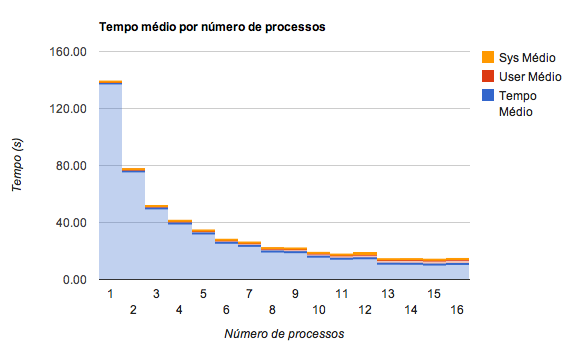
\includegraphics[width=0.97\linewidth]{img/grafico_tempos_aferidos}}
\caption{Gr�fico de tempos aferidos de acordo com o n�mero de processos}
\label{Fig:grafico_tempos_aferidos}
\end{center} \end{figure}